% GEODISC study report — Version 1 (2026-07-12)
% Supersedes manuscript.tex (v0 framework). Compile: pdflatex twice (manual thebibliography).
\documentclass[11pt]{article}
\usepackage[a4paper,margin=2.1cm]{geometry}
\usepackage[utf8]{inputenc}
\usepackage[round,authoryear]{natbib}
\usepackage{booktabs,amsmath,amssymb,mhchem,graphicx,caption,microtype,setspace,array}
\setstretch{1.0}
\captionsetup{font=small,labelfont=bf}
\title{\vspace{-1.0cm}\textbf{Silicification, not oxygenation: a compiled-record test of the
redox-preservation hypothesis for the Precambrian microfossil record}}
\author{[Author Name]\\
\small\textit{GEODISC -- Geological Discovery programme, [Institution]}}
\date{\small GEODISC study report, Version 1 (2026-07-12)}
\begin{document}
\maketitle

\begin{abstract}\small
\noindent Low atmospheric oxygen before the Great Oxidation Event (GOE, $\sim$2.4~Ga) should, in
principle, have slowed oxidative degradation of organic matter and favoured fossil preservation; yet
morphologically diagnostic microfossils are comparatively sparse before the GOE and diversify
afterwards. We tested the attractive interpretation that this pattern reflects a redox-driven shift
in preservation, by compiling published preservation, redox-proxy and silica-cycle data across the
GOE for six chert-hosted biotas (Strelley Pool, Moodies and Tumbiana, pre-GOE; Belcher, Gunflint and
Sokoman, post-GOE) and a cross-GOE shale redox compilation. Three findings reshape the question.
(1) Morphological fidelity tracks \emph{early silicification}, not the GOE: the pre-GOE Strelley
Pool biota is silica-encapsulated and morphology-rich, falsifying any simple pre/post-GOE contrast.
(2) The premise that the redox regime shifted cleanly across the GOE is not supported:
ferruginous conditions dominate on both sides in the global iron-speciation compilation. (3)
Seawater silica was supersaturated throughout the Precambrian and was not drawn down until the
Neoproterozoic--Phanerozoic radiation of biosilicifiers, so the silica cycle did not shift across
the GOE either. Together these reject the specific mechanisms proposed for a redox-driven
preservation shift (sulfate-enabled pyritisation; a GOE silica-cycle lever) and implicate
silicification---a facies/diagenetic variable largely decoupled from marine redox---as the dominant
control. We conclude that the apparent post-GOE ``rise'' of microfossils is primarily a
facies/sampling signal rather than an oxygenation signal, and we outline the narrower conditions
under which the GOE could still exert a second-order taphonomic influence.
\end{abstract}

\noindent\textbf{Keywords:} Great Oxidation Event; taphonomy; silicification; Precambrian microfossils;
iron speciation; silica cycle; kerogen; Raman spectroscopy.

%==================================================================
\section{Introduction}

Before the GOE, atmospheric \ce{O2} was below $\sim$$10^{-5}$~PAL --- low enough that
mass-independent sulfur isotope fractionation (S-MIF) was continuously expressed
\citep{Pavlov2002,Farquhar2000} --- and oceans were anoxic and ferruginous with seawater sulfate
$\lesssim$200~\textmu M \citep{Habicht2002,Crowe2014}. Under such conditions aerobic respiration,
the most efficient organic-matter degradation pathway, was suppressed. It is therefore tempting to
expect the Archean to have been a high-fidelity archive of early life, and equally tempting to read
the post-GOE diversification of the microfossil record \citep{Javaux2018,Wacey2014} as a
preservational---or biological---consequence of oxygenation. The two readings are not exclusive, and
distinguishing them is the deeper problem this paper addresses.

We began from a working hypothesis: that preservation of organic carbon and of morphology are
decoupled, and that the GOE-driven sulfate rise made microbial pyritisation newly available, so
that post-GOE morphology reflected a redox-enabled preservation pathway rather than biomass. This
report records what a compiled-record test of that hypothesis revealed, and how the hypothesis was
revised as a result. We treat the evolution of the interpretation as part of the scientific record
rather than disguising it: a hypothesis that survives empirical stress is worth more than one never
tested.

%==================================================================
\section{Background}

\subsection{The GOE and the redox landscape}
The GOE is pinned to $\sim$2.32--2.45~Ga by the disappearance of S-MIF
\citep{Bekker2004,Farquhar2003}, but was prolonged and oscillatory
\citep{Lyons2014,Garduno2024}, with proposed drivers including organic-carbon burial during the
Lomagundi--Jatuli excursion \citep{Bekker2012,Hodgskiss2023}, hydrogen escape \citep{Catling2001}
and a shift to subaerial volcanism \citep{Kump2007}. Mid-Proterozoic \ce{O2} was low
($\sim$1--10\%~PAL or $\le$0.1\%~PAL; \citealp{Lyons2014,Planavsky2014}) and the deep ocean
remained anoxic \citep{Canfield1998}. Local redox is reconstructed from iron speciation
\citep[$\mathrm{Fe_{HR}}/\mathrm{Fe_T}>0.38$;][]{Poulton2005,Poulton2011}, chromium isotopes
\citep{Frei2009} and Mo--U--N systematics \citep{Scott2008,Garvin2009}. Seawater sulfate rose across
the GOE from \textmu M to mM levels \citep{Habicht2002,Kah2004,Crowe2014}.

\subsection{The Precambrian microfossil record}
Archean microfossils are sparse and contested: the $\sim$3.46~Ga Apex chert structures
\citep{Schopf1993} were reinterpreted as abiogenic artefacts \citep{Brasier2002}, and many Archean
biotas are mat-related and morphologically simple. A widely noted pattern is that morphologically
diagnostic, taxonomically resolvable assemblages become abundant only after the GOE, peaking in the
Gunflint-type biotas at $\sim$1.9~Ga \citep{Javaux2018,Wacey2014}.

\subsection{Two preservation modes, and the mineral templating race}
Organic-carbon survival is governed by oxygen-exposure time, sedimentation rate, recalcitrance, and
mineral (iron-) surface protection \citep{Canfield1994,Hedges1995,Hartnett1998,Lalonde2012}.
Morphological fidelity, in contrast, is won or lost in a race between decay and early-diagenetic
mineral templating: cellular structure is preserved only when silica, pyrite, phosphate or clay
minerals impregnate or encrust cells \emph{before} decay collapses morphology \citep{Wacey2012}.
The two modes share decay as an antagonist but depend on different, independently variable mineral
pathways.

\subsection{Raman spectroscopy and the maturity control}
Raman spectroscopy of carbonaceous material (CM) provides both a peak-maturity geothermometer
\citep{Beyssac2002} (via $R_2=A_{D1}/(A_{D1}+A_{G1}+A_{G2})$) and a measure of CM structural order
aromaticity \citep{Qu2019}, allowing samples to be compared for thermal history and for the
structural imprint of differing preservation pathways.

\subsection{Silicification and the Precambrian silica cycle}
Silica entombment preserves labile molecular signatures \citep{Alleon2016silica} and underpins
exceptional preservation from the Archean to the Ediacaran \citep{Tarhan}. Critically, before the
evolution of biosilicifiers, Precambrian seawater was supersaturated with respect to amorphous
silica ($\sim$2~mM Si; $\geq$60~ppm \ce{SiO2}, versus $\sim$0.1~ppm today), with abiological
precipitation the dominant sink \citep{Siever1992,Perry2003}. The drawdown of dissolved silica is a
Neoproterozoic--Phanerozoic story --- driven by sponges, then radiolaria (Ordovician) and diatoms
(Mesozoic--Cenozoic) --- \emph{not} a GOE story (Table~\ref{tab:sicycle}).

%==================================================================
\section{Approach: a compiled-record test}

We compiled published preservation, redox and silica data across the GOE into two panels
(\texttt{data} available with the study). \textbf{Panel A}: six chert-hosted biotas spanning the
GOE, scored ordinally (0--3) for morphological fidelity, early silicification, and pyritisation
(sources in Fig.~\ref{fig:panel}). \textbf{Panel B}: a cross-GOE shale redox compilation
(\(\mathrm{Fe_{HR}}/\mathrm{Fe_T}\), \(\mathrm{Fe_{py}}/\mathrm{Fe_{HR}}\), sulfate/trace-metal
proxies). We treat the scores as hypothesis-generating, not statistical, and report gaps honestly.
All entries are sourced; no values were estimated.

%==================================================================
\section{Findings}

\subsection{Morphological fidelity tracks silicification, not the GOE}

Across all six biotas, morphological fidelity co-varies with early silica encapsulation and is
uncorrelated with GOE side (Fig.~\ref{fig:panel}). The decisive counter-example to a GOE/redox
driver is \textbf{Strelley Pool} ($\sim$3.4~Ga, $\sim$1~Gyr before the GOE): silica-encapsulated,
Raman $\sim$300~$^\circ$C, and morphology-rich (lenticular forms, chains/clusters, and
``tail-like'' microfossils; \citealp{Delarue2020,Delarue2021,Sugitani2010}). If redox/GOE drove
morphological richness, Strelley Pool should be poor; it is not. Conversely, the pre-GOE Tumbiana
and Moodies biotas are morphology-poor precisely where silica entombment is weak or absent
(carbonate-hosted globules; siliciclastic mats; \citealp{Lepot2009,Homann2015,Decreane2021}). The
post-GOE Gunflint, Sokoman and Belcher biotas are silica-encapsulated and morphology-rich
\citep{Lepot2017,Hodgskiss2020}. Where preservation is resolved at the nanoscale (Gunflint), the
preservative pathway is explicitly early silicification plus Fe-biomineralization
\citep{Lepot2017,Alleon2016}.

\begin{figure}[t]
\centering
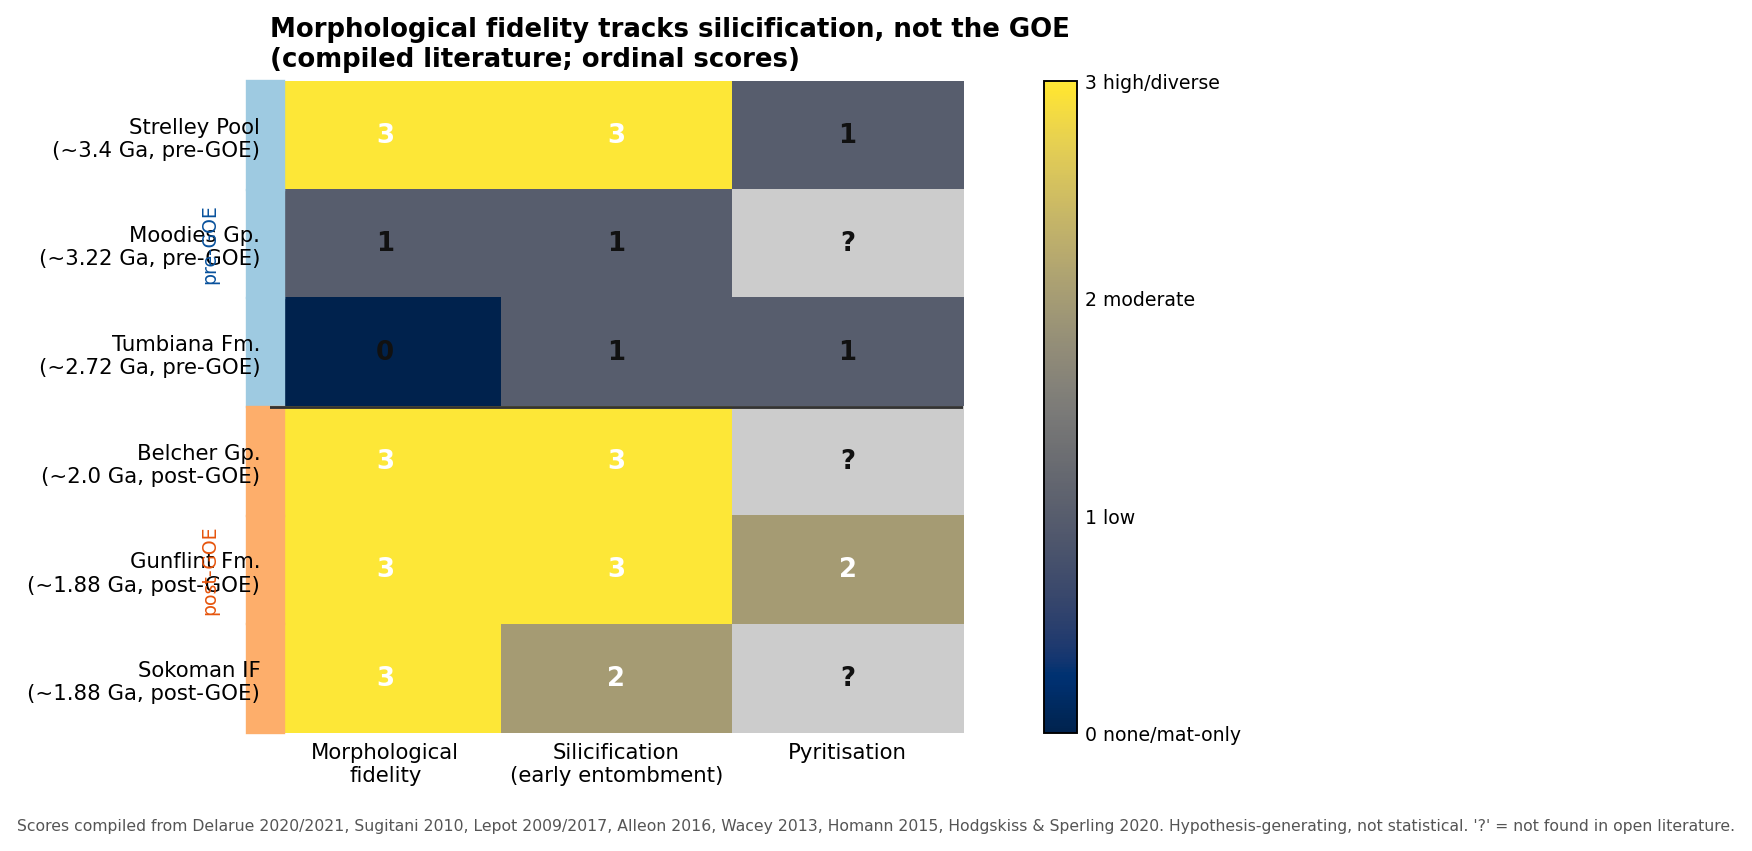
\includegraphics[width=0.92\linewidth]{fig_panel.png}
\caption{Compiled literature scores (0--3; grey = ``?'' not found) for six chert-hosted biotas.
Morphological fidelity and silicification columns share the same pattern; the GOE side does not.
Scores compiled from \citep{Delarue2020,Delarue2021,Sugitani2010,Lepot2009,Decreane2021,
Lepot2017,Alleon2016,Wacey2013,Homann2015,Hodgskiss2020}. Ordinal and hypothesis-generating, not
statistical.}
\label{fig:panel}
\end{figure}

\subsection{Pyritisation is destructive, not preservative, in the best-preserved biotas}

In Gunflint, pyritisation occurs in scarce patches, in a locally sulfate-limited setting, and
``nearly obliterates organic structures'' \citep{Wacey2013,Lepot2017}; the preserved morphologies
carry intra-cellular greenalite + siderite, not pyrite \citep{Lepot2017}. Pyritisation also occurred
pre-GOE (Tumbiana micropyrites and bacterial-sulfate-reduction-driven sulfurization;
\citealp{Decreane2021,Lepot2009}). The original sulfate$\to$pyritisation mechanism is therefore
rejected on three independent grounds: pyritisation is pre-GOE, locally sulfate-limited even
post-GOE, and destructive where it occurs.

\subsection{The redox regime did not shift cleanly across the GOE}

The cross-GOE shale record does not show an uncontested redox shift. Ferruginous conditions dominate
on both sides of the GOE, euxinia is spatially variable (e.g.\ Barney Creek photic euxinia,
\citealp{Sperling2014}; Mt McRae transient ``whiffs'', \citealp{Anbar2007}), and the global
compilation shows ferruginous conditions dominating on both sides (no clean anoxic-to-oxic
transition at the GOE; \citealp{Poulton2011,Sperling2014}). The redox shift cannot therefore be
assumed as the independent variable; it is itself a hypothesis, and one that diagenetic
overprinting can further obscure.

\subsection{The silica cycle did not shift across the GOE either}

\begin{table}[t]
\centering\small
\caption{Secular state of the marine silica cycle. The GOE (2.4~Ga) sits entirely within the
high-silica Precambrian regime; the drawdown is a much later, biologically driven event.
After \citep{Siever1992,Perry2003,ESR2023Si}.}
\label{tab:sicycle}
\begin{tabular}{llll}
\toprule
Interval & Seawater DSi & Dominant Si sink & GOE relevance \\
\midrule
Archean--Proterozoic & supersaturated ($\sim$2~mM) & abiological (chert, Fe-oxide/clay adsorption) & high on both sides of GOE \\
Neoproterozoic--early Palaeozoic & beginning to decline & early sponges, first radiolaria & post-dates GOE by $>$1.5~Gyr \\
Palaeozoic--Mesozoic & substantially drawn down & radiolaria, sponges; diatoms rise & post-dates GOE \\
Cenozoic--modern & $\sim$0.1~ppm & diatoms ($\sim$75\% of biogenic Si burial) & --- \\
\bottomrule
\end{tabular}
\end{table}

Because seawater silica was high throughout the Precambrian, the GOE could not have ``switched on''
silicification capacity. Any revised mechanism invoking a GOE silica-cycle lever therefore also
fails: silicification \emph{capacity} was available before and after the GOE alike.

%==================================================================
\section{Revised interpretation}

The compiled-record test rejects both candidate GOE mechanisms --- sulfate-enabled pyritisation
(\S4.2) and a GOE silica-cycle switch (\S4.4) --- while supporting the more general claim that
morphological fidelity is gated by early silica encapsulation (\S4.1). The inescapable conclusion is
that the GOE is \emph{not} the primary control on microfossil morphological preservation. Because
silica entombment capacity was high on both sides of the GOE, the variation in fidelity across the
record is governed by \emph{which facies received early silicification} (a local depositional and
early-diagenetic control: peritidal concentration, ferruginous silica precipitation, microbial
silica nucleation), not by oxygenation. The apparent post-GOE ``rise'' of morphological microfossils
is therefore most parsimoniously read as a facies and rock-volume/sampling signal, amplified where
silica-encapsulating shallow-marine cherts are well-exposed and well-sampled (Gunflint, Belcher),
rather than as a biological or redox signal.

We do not claim the GOE is taphonomically irrelevant. Two second-order channels remain plausible.
First, the GOE changed the \emph{decay community} (more \ce{O2}, more sulfate post-GOE), altering
the rate and selectivity of organic-matter degradation; but where silicification outpaced decay
in silica-rich facies --- as at pre-GOE Strelley Pool --- this difference would not surface as a
morphology contrast. Second, sulfate and the OM-sulfurization balance affect \emph{what} organic
matter survives (the S-poor/S-rich OM pools of Tumbiana, \citealp{Lepot2009}), influencing bulk
kerogen character more than cellular fidelity. Both are quantifiable but neither is the dominant
signal in the present compilation.

%==================================================================
\section{Implications}

\textbf{Reading the fossil record.} Treating microfossil abundance or diversity as a direct proxy
for biomass or biological innovation across the GOE is unreliable without accounting for the
silicification/facies control. Quantitative estimates of Proterozoic diversity should be
facies-corrected, not redox-corrected alone.

\textbf{Unmasking versus evolution.} The richness of OM in pre-GOE units without diagnostic
morphology (Tumbiana globules; Moodies mats) is consistent with \emph{latent, morphologically
invisible} diversity; resolving whether post-GOE morphological novelty reflects evolution or
unmasking still requires independent temporal evidence (molecular clocks, biomarkers), as recently
emphasised in critiques of framework papers of this type.

\textbf{Biosignatures on Mars and early Earth.} The absence of morphological microfossils in an
anoxic, poorly silicified succession does not entail the absence of life; the requisite variable
is a silica-encapsulating facies, not oxygen.

%==================================================================
\section{Conclusions}

A compiled-record test across the GOE falsifies the redox-preservation hypothesis in its specific
forms: morphological fidelity tracks early silicification, not the GOE (pre-GOE Strelley Pool is
morphology-rich); pyritisation is pre-GOE, locally sulfate-limited, and destructive; the bulk-redox
shift across the GOE is itself contested; and the silica cycle did not shift across the GOE. The
post-GOE ``rise'' of microfossils is best read as a facies/sampling signal rather than an
oxygenation signal. The work illustrates the value of subjecting an attractive taphonomic narrative
to an empirical, fiction-free compiled-record test before drawing biological or redox conclusions
from first appearances. The narrower question of how the GOE reshaped decay and OM-sulfurisation
remains open and is the appropriate focus of targeted new measurement.

%==================================================================
\bibliographystyle{plainnat}
\begin{thebibliography}{99}\footnotesize\linespread{0.92}\selectfont\setlength{\itemsep}{0pt}\setlength{\parskip}{0pt}
\bibitem[Alleon et al.(2016)]{Alleon2016silica} Alleon, J., et al. (2016). Early entombment within
silica minimizes the molecular degradation of microorganisms during advanced diagenesis.
\textit{Chemical Geology}.
\bibitem[Alleon et al.(2016a)]{Alleon2016} Alleon, J., et al. (2016). Molecular preservation of
1.88~Ga Gunflint organic microfossils as a function of temperature and mineralogy. \textit{Nature
Communications} 7, 11977.
\bibitem[Anbar et al.(2007)]{Anbar2007} Anbar, A.~D., et al. (2007). A whiff of oxygen before the
Great Oxidation Event? \textit{Science} 317, 1903--1906.
\bibitem[Bekker et al.(2004)]{Bekker2004} Bekker, A., et al. (2004). Dating the rise of atmospheric
oxygen. \textit{Nature} 427, 117--120.
\bibitem[Bekker \& Holland(2012)]{Bekker2012} Bekker, A., \& Holland, H.~D. (2012). Oxygen overshoot
and recovery during the early Paleoproterozoic. \textit{Earth Planet. Sci. Lett.} 317--318, 295--304.
\bibitem[Beyssac et al.(2002)]{Beyssac2002} Beyssac, O., et al. (2002). Raman spectra of
carbonaceous material in metasediments: a new geothermometer. \textit{J. Metamorph. Geol.} 20,
859--871.
\bibitem[Brasier et al.(2002)]{Brasier2002} Brasier, M.~D., et al. (2002). Questioning the evidence
for Earth's oldest fossils. \textit{Nature} 416, 76--81.
\bibitem[Canfield(1994)]{Canfield1994} Canfield, D.~E. (1994). Factors influencing organic carbon
preservation in marine sediments. \textit{Chem. Geol.} 114, 315--329.
\bibitem[Canfield(1998)]{Canfield1998} Canfield, D.~E. (1998). A new model for Proterozoic ocean
chemistry. \textit{Nature} 396, 450--453.
\bibitem[Catling et al.(2001)]{Catling2001} Catling, D.~C., Zahnle, K.~J., \& McKay, C.~P. (2001).
Biogenic methane, hydrogen escape, and the irreversible oxidation of early Earth. \textit{Science}
293, 839--843.
\bibitem[Crowe et al.(2014)]{Crowe2014} Crowe, S.~A., et al. (2014). Sulfate was a trace constituent
of the Archean ocean. \textit{Science} 346, 735--739.
\bibitem[Decreane et al.(2021)]{Decreane2021} Decreane, S., et al. (2021). Intense biogeochemical
iron cycling revealed in Neoarchean Tumbiana Formation stromatolites. \textit{Geochim. Cosmochim.
Acta} (in-situ Fe isotopes of micropyrites).
\bibitem[Delarue et al.(2020)]{Delarue2020} Delarue, F., et al. (2020). Out of rock: a new look at
the morphological and geochemical preservation of microfossils from the 3.46~Gyr-old Strelley Pool
Formation. \textit{Precambrian Research} 336, 105472.
\bibitem[Delarue et al.(2021)]{Delarue2021} Delarue, F., et al. (2021). Microfossils with tail-like
structures in the 3.4~Gyr old Strelley Pool Formation. \textit{Organic Geochemistry}.
\bibitem[Farquhar et al.(2000)]{Farquhar2000} Farquhar, J., Bao, H., \& Thiemens, M. (2000).
Atmospheric influence of Earth's earliest sulfur cycle. \textit{Science} 289, 756--758.
\bibitem[Farquhar \& Wing(2003)]{Farquhar2003} Farquhar, J., \& Wing, B.~A. (2003). Multiple sulfur
isotopes and the evolution of the atmosphere. \textit{Earth Planet. Sci. Lett.} 213, 1--13.
\bibitem[Frei et al.(2009)]{Frei2009} Frei, R., et al. (2009). Fluctuations in Precambrian
atmospheric oxygenation recorded by chromium isotopes. \textit{Nature} 461, 250--253.
\bibitem[Gardu\~{n}o Ruiz et al.(2024)]{Garduno2024} Gardu\~{n}o Ruiz, D., Goldblatt, C., \& Ahm,
A.-S.~C. (2024). Climate variability leads to multiple oxygenation episodes across the GOE.
\textit{Geophys. Res. Lett.} 51, e2023GL106694.
\bibitem[Garvin et al.(2009)]{Garvin2009} Garvin, J., et al. (2009). Isotopic evidence for an
aerobic nitrogen cycle in the latest Archean. \textit{Science} 323, 1045--1048.
\bibitem[Habicht et al.(2002)]{Habicht2002} Habicht, K.~S., et al. (2002). Calibration of sulfate
levels in the Archean ocean. \textit{Science} 298, 2372--2374.
\bibitem[Hartnett et al.(1998)]{Hartnett1998} Hartnett, H.~E., et al. (1998). Influence of oxygen
exposure time on organic carbon preservation. \textit{Nature} 391, 572--575.
\bibitem[Hedges \& Keil(1995)]{Hedges1995} Hedges, J.~I., \& Keil, R.~G. (1995). Sedimentary organic
matter preservation. \textit{Mar. Chem.} 49, 81--115.
\bibitem[Hodgskiss \& Sperling(2020)]{Hodgskiss2020} Hodgskiss, M.~S.~W., \& Sperling, E.~A. (2020).
Stratigraphy and shale geochemistry of the Belcher Group.
\bibitem[Hodgskiss et al.(2023)]{Hodgskiss2023} Hodgskiss, M.~S.~W., Crockford, P.~W., \& Turchyn,
A. (2023). Deconstructing the Lomagundi--Jatuli carbon isotope excursion. \textit{Annu. Rev. Earth
Planet. Sci.} 51, 301--330.
\bibitem[Homann et al.(2015)]{Homann2015} Homann, M., et al. (2015). Morphological adaptations of
3.22~Ga-old tufted microbial mats, Moodies Group. \textit{Precambrian Research}.
\bibitem[Javaux et al.(2018)]{Javaux2018} Javaux, E.~J., Lepot, K., \& Knoll, A.~H. (2018). The
Paleoproterozoic fossil record. \textit{Earth-Science Reviews}.
\bibitem[Kah et al.(2004)]{Kah2004} Kah, L.~C., Lyons, T.~W., \& Frank, T.~D. (2004). Low marine
sulfate and protracted oxygenation of the Proterozoic biosphere. \textit{Nature} 431, 834--838.
\bibitem[Kump \& Barley(2007)]{Kump2007} Kump, L.~R., \& Barley, M.~E. (2007). Increased subaerial
volcanism and the rise of atmospheric oxygen. \textit{Nature} 448, 1033--1036.
\bibitem[Lalonde et al.(2012)]{Lalonde2012} Lalonde, K., et al. (2012). Preservation of organic
matter in sediments promoted by iron. \textit{Nature} 483, 198--200.
\bibitem[Lepot et al.(2009)]{Lepot2009} Lepot, K., et al. (2009). Organic matter heterogeneities in
2.72~Ga stromatolites: alteration versus preservation by sulfur incorporation. \textit{Geochim.
Cosmochim. Acta} 73, 6579--6599.
\bibitem[Lepot et al.(2017)]{Lepot2017} Lepot, K., et al. (2017). Iron minerals within specific
microfossil morphospecies of the 1.88~Ga Gunflint Formation. \textit{Nature Communications} 8, 14890.
\bibitem[Lyons et al.(2014)]{Lyons2014} Lyons, T.~W., Reinhard, C.~T., \& Planavsky, N.~J. (2014).
The rise of oxygen in Earth's early ocean and atmosphere. \textit{Nature} 506, 307--315.
\bibitem[Pavlov \& Kasting(2002)]{Pavlov2002} Pavlov, A.~A., \& Kasting, J.~F. (2002).
Mass-independent fractionation of sulfur isotopes in Archean sediments. \textit{Astrobiology} 2,
27--41.
\bibitem[Perry \& Lefticariu(2003)]{Perry2003} Perry, E.~C., \& Lefticariu, P. (2003). Formation and
geochemistry of Precambrian cherts. \textit{Treatise on Geochemistry} 7, 99--113.
\bibitem[Planavsky et al.(2014)]{Planavsky2014} Planavsky, N.~J., et al. (2014). Low
mid-Proterozoic atmospheric oxygen levels and the delayed rise of animals. \textit{Science} 346,
635--638.
\bibitem[Poulton \& Canfield(2005)]{Poulton2005} Poulton, S.~W., \& Canfield, D.~E. (2005).
Development of a sequential extraction procedure for iron. \textit{Chem. Geol.} 214, 209--221.
\bibitem[Poulton \& Canfield(2011)]{Poulton2011} Poulton, S.~W., \& Canfield, D.~E. (2011).
Ferruginous conditions: a dominant feature of the ocean through Earth's history. \textit{Elements}
7, 107--112.
\bibitem[Qu et al.(2019)]{Qu2019} Qu, Y., Bower, D.~M., et al. (2019). Raman spectroscopy and
structural heterogeneity of carbonaceous matter in Precambrian microfossils. \textit{Org. Geochem.}
\bibitem[Schopf(1993)]{Schopf1993} Schopf, J.~W. (1993). Microfossils of the Early Archean Apex
chert. \textit{Science} 260, 640--646.
\bibitem[Scott et al.(2008)]{Scott2008} Scott, C., et al. (2008). Tracing the stepwise oxygenation
of the Proterozoic ocean. \textit{Nature} 452, 456--459.
\bibitem[Siever(1992)]{Siever1992} Siever, R. (1992). The silica cycle in the Precambrian.
\textit{Geochim. Cosmochim. Acta} 56, 3265--3272.
\bibitem[Sperling et al.(2014)]{Sperling2014} Sperling, E.~A., et al. (2014). Redox heterogeneity of
subsurface waters in the Mesoproterozoic ocean. \textit{Geobiology}.
\bibitem[Sugitani et al.(2010)]{Sugitani2010} Sugitani, K., et al. (2010). Biogenicity of
morphologically diverse carbonaceous microfossils from the $\sim$3.4~Ga Strelley Pool Formation.
\bibitem[Tarhan et al.(2016)]{Tarhan} Tarhan, L.~G., et al. (2016). Exceptional preservation of
soft-bodied Ediacara Biota promoted by early silicification. \textit{Geology}.
\bibitem[Wacey et al.(2012)]{Wacey2012} Wacey, D., et al. (2012). Taphonomy of very ancient
microfossils from the $\sim$3400~Ma Strelley Pool Formation and $\sim$1900~Ma Gunflint Formation.
\textit{Precambrian Research}.
\bibitem[Wacey et al.(2013)]{Wacey2013} Wacey, D., et al. (2013). Nanoscale analysis of pyritized
microfossils reveals differential heterotrophic consumption in the $\sim$1.9~Ga Gunflint chert.
\textit{PNAS} 110, 8020--8024.
\bibitem[Wacey et al.(2014)]{Wacey2014} Wacey, D., et al. (2014). Changing the picture of Earth's
earliest fossils (3.5--1.9~Ga). \textit{PNAS} 111.
\bibitem[Earth-Science Reviews(2023)]{ESR2023Si} The evolution of the marine Si cycle in the
Archean--Palaeozoic. \textit{Earth-Science Reviews} (2023).
\end{thebibliography}

\end{document}
